%%%%%%%%%%%%%%%%%%%%%%%%%%%%%%%%%%%%%%%%%
% Programming/Coding Assignment
% LaTeX Template
%
% This template has been downloaded from:
% http://www.latextemplates.com
%
% Original author:
% Ted Pavlic (http://www.tedpavlic.com)
%
% Note:
% The \lipsum[#] commands throughout this template generate dummy text
% to fill the template out. These commands should all be removed when 
% writing assignment content.
%
% This template uses a Perl script as an example snippet of code, most other
% languages are also usable. Configure them in the "CODE INCLUSION 
% CONFIGURATION" section.
%
%%%%%%%%%%%%%%%%%%%%%%%%%%%%%%%%%%%%%%%%%

%----------------------------------------------------------------------------------------
%	PACKAGES AND OTHER DOCUMENT CONFIGURATIONS
%----------------------------------------------------------------------------------------

\documentclass{article}

\usepackage{float}
\usepackage{fancyhdr} % Required for custom headers
\usepackage{lastpage} % Required to determine the last page for the footer
\usepackage{extramarks} % Required for headers and footers
\usepackage[usenames,dvipsnames]{color} % Required for custom colors
\usepackage{graphicx} % Required to insert images
\usepackage{listings} % Required for insertion of code
\usepackage{courier} % Required for the courier font
\usepackage{lipsum} % Used for inserting dummy 'Lorem ipsum' text into the template
\usepackage{amsmath}
\usepackage{amssymb}
\usepackage{textcomp}
\usepackage{subcaption}
\usepackage{multirow}


% Margins
\topmargin=-0.45in
\evensidemargin=0in
\oddsidemargin=0in
\textwidth=6.5in
\textheight=9.0in
\headsep=0.25in

\linespread{1.1} % Line spacing

% Set up the header and footer
\pagestyle{fancy}
\lhead{\hmwkAuthorName} % Top left header
\chead{\hmwkClass\ : \hmwkTitle} % Top center head
\rhead{\firstxmark} % Top right header
\lfoot{\lastxmark} % Bottom left footer
\cfoot{} % Bottom center footer
\rfoot{Page\ \thepage\ of\ \protect\pageref{LastPage}} % Bottom right footer
\renewcommand\headrulewidth{0.4pt} % Size of the header rule
\renewcommand\footrulewidth{0.4pt} % Size of the footer rule

\setlength\parindent{0pt} % Removes all indentation from paragraphs

%----------------------------------------------------------------------------------------
%	CODE INCLUSION CONFIGURATION
%----------------------------------------------------------------------------------------

\definecolor{MyDarkGreen}{rgb}{0.0,0.4,0.0} % This is the color used for comments
\lstloadlanguages{Perl} % Load Perl syntax for listings, for a list of other languages supported see: ftp://ftp.tex.ac.uk/tex-archive/macros/latex/contrib/listings/listings.pdf
\lstset{language=Perl, % Use Perl in this example
        frame=single, % Single frame around code
        basicstyle=\small\ttfamily, % Use small true type font
        keywordstyle=[1]\color{Blue}\bf, % Perl functions bold and blue
        keywordstyle=[2]\color{Purple}, % Perl function arguments purple
        keywordstyle=[3]\color{Blue}\underbar, % Custom functions underlined and blue
        identifierstyle=, % Nothing special about identifiers                                         
        commentstyle=\usefont{T1}{pcr}{m}{sl}\color{MyDarkGreen}\small, % Comments small dark green courier font
        stringstyle=\color{Purple}, % Strings are purple
        showstringspaces=false, % Don't put marks in string spaces
        tabsize=5, % 5 spaces per tab
        %
        % Put standard Perl functions not included in the default language here
        morekeywords={rand},
        %
        % Put Perl function parameters here
        morekeywords=[2]{on, off, interp},
        %
        % Put user defined functions here
        morekeywords=[3]{test},
       	%
        morecomment=[l][\color{Blue}]{...}, % Line continuation (...) like blue comment
        numbers=left, % Line numbers on left
        firstnumber=1, % Line numbers start with line 1
        numberstyle=\tiny\color{Blue}, % Line numbers are blue and small
        stepnumber=5 % Line numbers go in steps of 5
}

% Creates a new command to include a perl script, the first parameter is the filename of the script (without .pl), the second parameter is the caption
\newcommand{\perlscript}[2]{
\begin{itemize}
\item[]\lstinputlisting[caption=#2,label=#1]{#1.pl}
\end{itemize}
}

%----------------------------------------------------------------------------------------
%	DOCUMENT STRUCTURE COMMANDS
%	Skip this unless you know what you're doing
%----------------------------------------------------------------------------------------

% Header and footer for when a page split occurs within a problem environment
\newcommand{\enterProblemHeader}[1]{
\nobreak\extramarks{#1}{#1 continued on next page\ldots}\nobreak
\nobreak\extramarks{#1 (continued)}{#1 continued on next page\ldots}\nobreak
}

% Header and footer for when a page split occurs between problem environments
\newcommand{\exitProblemHeader}[1]{
\nobreak\extramarks{#1 (continued)}{#1 continued on next page\ldots}\nobreak
\nobreak\extramarks{#1}{}\nobreak
}

\setcounter{secnumdepth}{0} % Removes default section numbers
\newcounter{homeworkProblemCounter} % Creates a counter to keep track of the number of problems
\newcounter{homeworkSubProblemCounter}

\newcommand{\homeworkProblemName}{}
\newenvironment{homeworkProblem}[1][Problem \arabic{homeworkProblemCounter}]{ % Makes a new environment called homeworkProblem which takes 1 argument (custom name) but the default is "Problem #"
\stepcounter{homeworkProblemCounter} % Increase counter for number of problems
\setcounter{homeworkSubProblemCounter}{0}
\renewcommand{\homeworkProblemName}{#1} % Assign \homeworkProblemName the name of the problem
\section{\homeworkProblemName} % Make a section in the document with the custom problem count
\enterProblemHeader{\homeworkProblemName} % Header and footer within the environment
}{
\exitProblemHeader{\homeworkProblemName} % Header and footer after the environment
}

\newcommand{\homeworkSubProblemName}{}
\newenvironment{homeworkSubProblem}[1][\arabic{homeworkProblemCounter}.\arabic{homeworkSubProblemCounter}]{ % Makes a new environment called homeworkSubProblem which takes 1 argument (custom name) but the default is "#.#"
\stepcounter{homeworkSubProblemCounter} % Increase counter for number of subproblems
\renewcommand{\homeworkSubProblemName}{#1} % Assign \homeworkSubProblemName the name of the problem
\subsection{\homeworkSubProblemName}
}

\newcommand{\problemAnswer}[1]{ % Defines the problem answer command with the content as the only argument
\noindent\framebox[\columnwidth][c]{\begin{minipage}{0.98\columnwidth}#1\end{minipage}} % Makes the box around the problem answer and puts the content inside
}

\newcommand{\homeworkSectionName}{}
\newenvironment{homeworkSection}[1]{ % New environment for sections within homework problems, takes 1 argument - the name of the section
\renewcommand{\homeworkSectionName}{#1} % Assign \homeworkSectionName to the name of the section from the environment argument
\subsection{\homeworkSectionName} % Make a subsection with the custom name of the subsection
\enterProblemHeader{\homeworkProblemName\ [\homeworkSectionName]} % Header and footer within the environment
}{
\enterProblemHeader{\homeworkProblemName} % Header and footer after the environment
}

%----------------------------------------------------------------------------------------
%	NAME AND CLASS SECTION
%----------------------------------------------------------------------------------------

\newcommand{\hmwkTitle}{Assignment 2} % Assignment title
\newcommand{\hmwkDueDate}{\ Wednessday,\ December\ 13th,\ 2017} % Due date
\newcommand{\hmwkClass}{VIP} % Course/class
\newcommand{\hmwkClassTime}{|TIME|} % Class/lecture time
\newcommand{\hmwkClassInstructor}{|INSTRUCTORNAME|} % Teacher/lecturer
\newcommand{\hmwkAuthorName}{Therese Darum, zbl558; Cecilie Novak, bqk662; Christoffer Belhage, DZP300} % Your name

%----------------------------------------------------------------------------------------
%	TITLE PAGE
%----------------------------------------------------------------------------------------

\title{
\vspace{2in}
\textmd{\textbf{\hmwkClass:\ \hmwkTitle}}\\
\normalsize\vspace{0.1in}\small{Due\ on\ \hmwkDueDate}\\
%\vspace{0.1in}\large{\textit{\hmwkClassInstructor\ \hmwkClassTime}}
\vspace{3in}
}

\author{\textbf{\hmwkAuthorName}}
\date{} % Insert date here if you want it to appear below your name

%----------------------------------------------------------------------------------------

\begin{document}

\maketitle

%----------------------------------------------------------------------------------------
%	TABLE OF CONTENTS
%----------------------------------------------------------------------------------------

%\setcounter{tocdepth}{1} % Uncomment this line if you don't want subsections listed in the ToC

\newpage
\tableofcontents
\newpage



%----------------------------------------------------------------------------------------
%	PROBLEM 1
%----------------------------------------------------------------------------------------
\begin{homeworkProblem}[Quick Intro]
...
\end{homeworkProblem}

\begin{homeworkProblem}[1: Detecting interest points (Features)]
For the assignment we have chosen to use the Harris corner detector. The implementation has been made by Cecilie for her bachelor's project back in 2016. More precisely, two files with code has been borrowed from this project: \textit{Harris\_corner\_function.m} and \textit{nms.m}.

\begin{homeworkSubProblem}[Implementation]
The Harris corner detector has been implemented in the file \textit{Harris\_corner\_function.m} using gaussian derivatives for the smoothing of the images, prior to the corner detection. \\\\
The computation of the Harris corner measures are implemented as in the original paper on the detector (making use of the constant $k = 0.04$). After computing the Harris measures, non-maxima suppression and thresholding is performed on the Harris measures, such that corners are only detected once and vaque corners, which possibly could be other structures than corners, are thrown away. The non-maximal suppression has been implemented separately in the file \textit{nms.m}. \\\\
The threshold used for discarding vague corners has been set as a parameter that specifies how big a measure must be relatively to the maximal Harris measure in the image (i.e., if the threshold parameter is set to $t = 0.5$, only measures bigger than half the maximal Harris measure in the image is kept). 
\end{homeworkSubProblem}

\begin{homeworkSubProblem}[Experimentation and results]
...
\end{homeworkSubProblem}

\end{homeworkProblem}

%----------------------------------------------------------------------------------------
%	PROBLEM 2
%----------------------------------------------------------------------------------------

\begin{homeworkProblem}[2: Simple matching of features]

\begin{homeworkSubProblem}[Implementation]

\textbf{Extracting points}\\
For each detected point of interest we must extract information to be used as a descriptor. The most simple extraction is placing a square $N\times N$ window centered over the detected pixel and using every pixel within the window as a descriptor. We pad the image with $N$ zeros, in case we wish to extract a descriptor from a pixel less than $\lfloor \frac{N}{2}\rfloor$ pixels from the border. Then for every extracted image patch we reshape it into a $N\cdot N$ vector. Every vector is then collected and placed into a matrix.\\

\textbf{Matching}\\
The matching was performed by calculating the difference between all the descriptors across the two images, using sum of squared intensity difference:
$$SSID(u,v) = \sum_{i=1}^{n}(u_i-v_i)^2$$
Then for each descriptor in the first image, the descriptor from the second image with the smallest difference is logged as the "match".\\
Just doing this produced a lot of unwanted matches, so we needed to filter the matches. Besides, multiple descriptors from the first image might match a single descriptor from the second image, which naturally does not make sense.\\
The first filtering applied is checking whether the second best match for any given descriptor is within some scale of the same difference to the best match. So, if the second best match is not far worse than the best match, then we consider the matches too ambiguous and discard it entirely.\\
This reduced the number of matches, depending on what scale was used to determine "too ambigous".\\
The next filter added is doing the exact same as described above, but for all descriptors in the second imaged compared to the descriptors in the first image. If a descriptor from the first image points to a descriptor from the second image, which in turn points to the same descriptor in the first image, then it is kept as a match, else discarded. That it, descriptors must match two-way.\\
Lastly, as a variable parameter, a hard threshold for how similar the matches should be before we keep them. This might be a less useful filter than the previous two; The statistics will show whether this is the case.

\end{homeworkSubProblem}

\clearpage
\begin{homeworkSubProblem}[Experimentation and results]
\textbf{Matchings}\\

\begin{figure}[H]
\centering
\begin{subfigure}[b]{1\textwidth}
	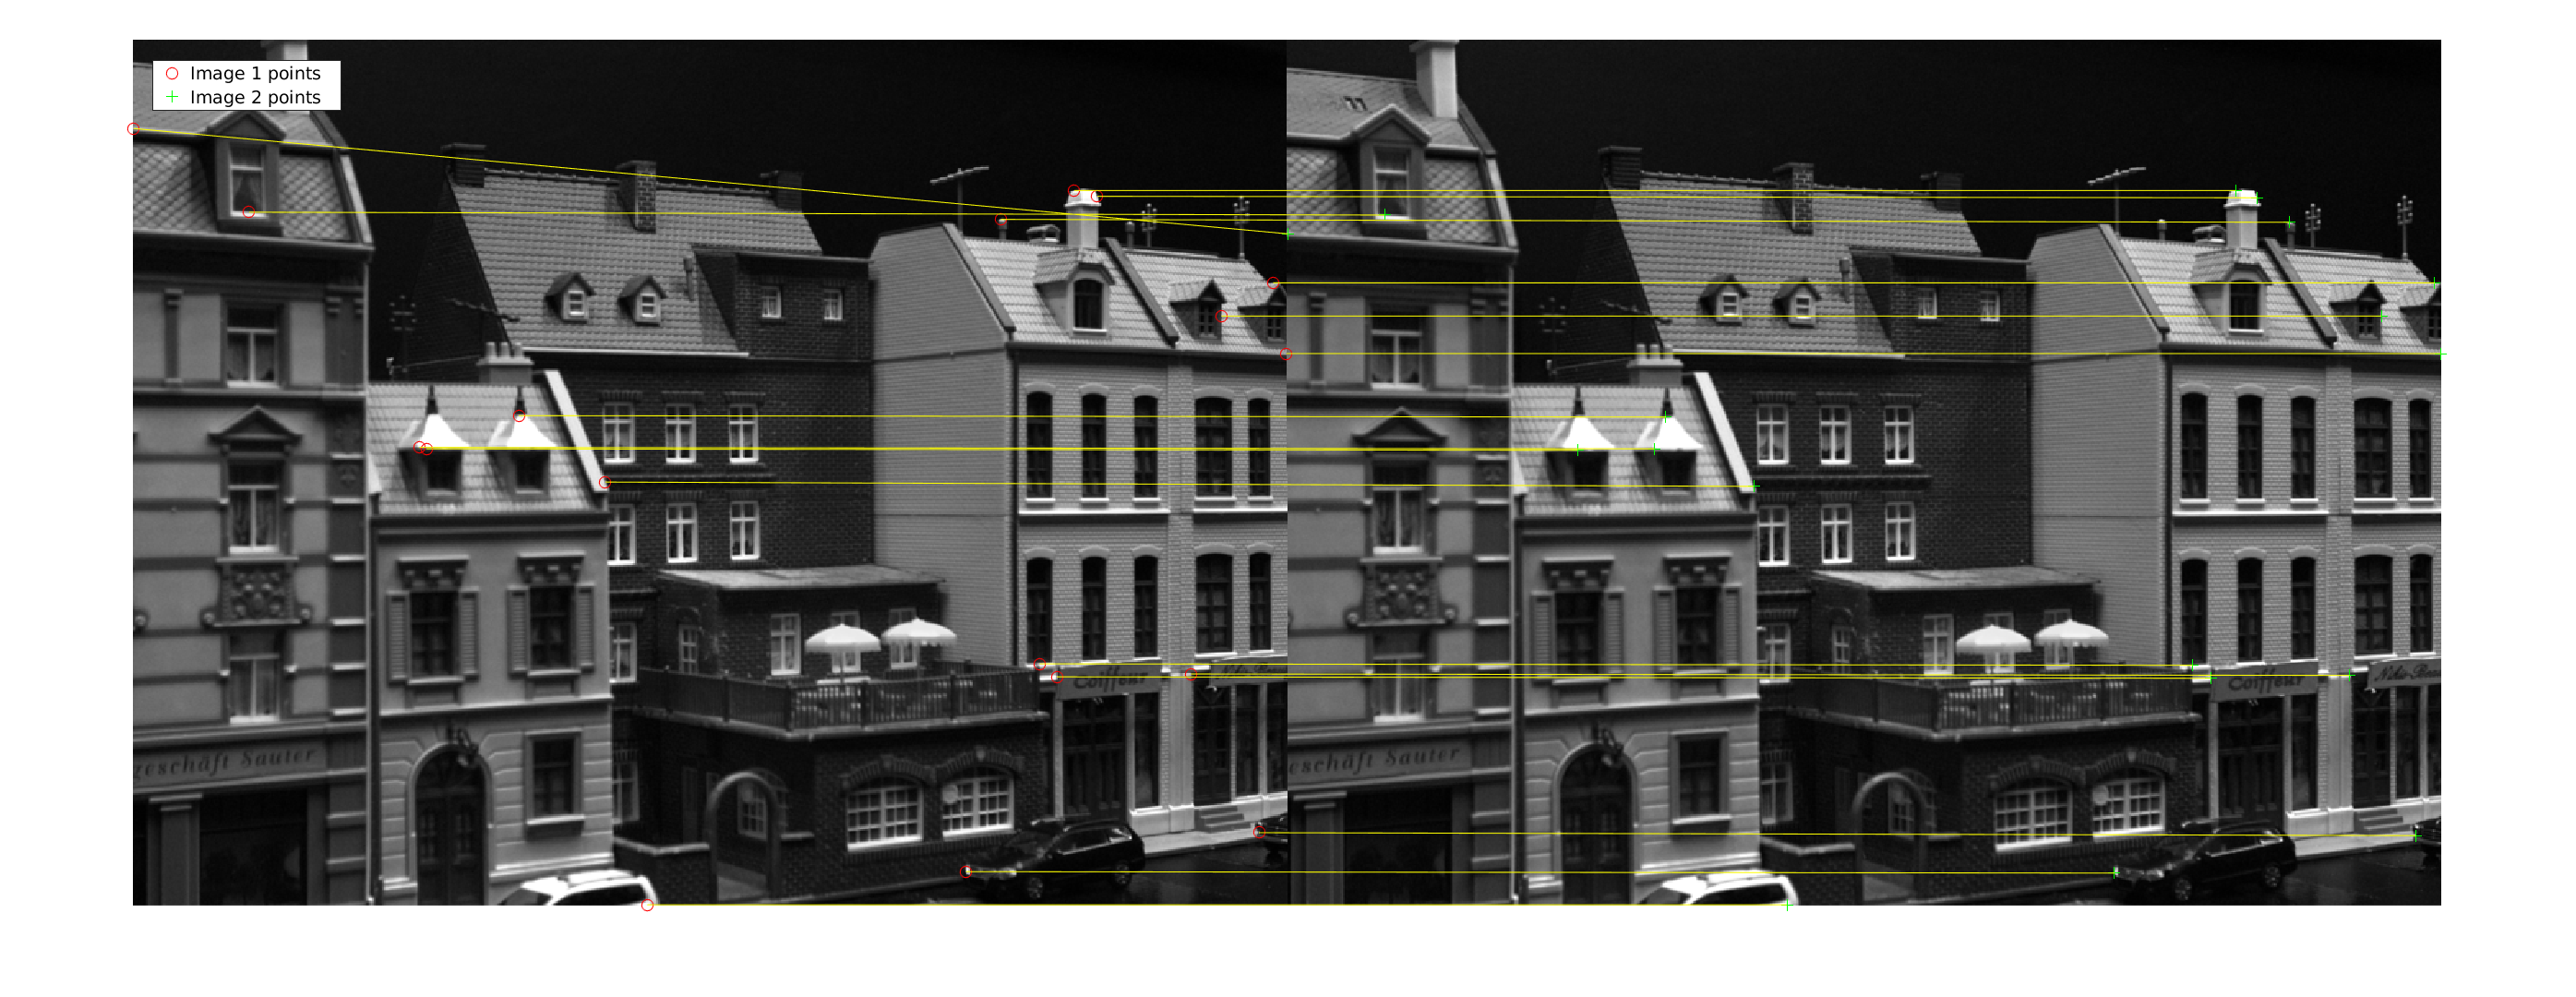
\includegraphics[width=\textwidth]{output/matches5.png}
	\caption{Using descriptor field width / height 5}
\end{subfigure}\\
\begin{subfigure}[b]{1\textwidth}
	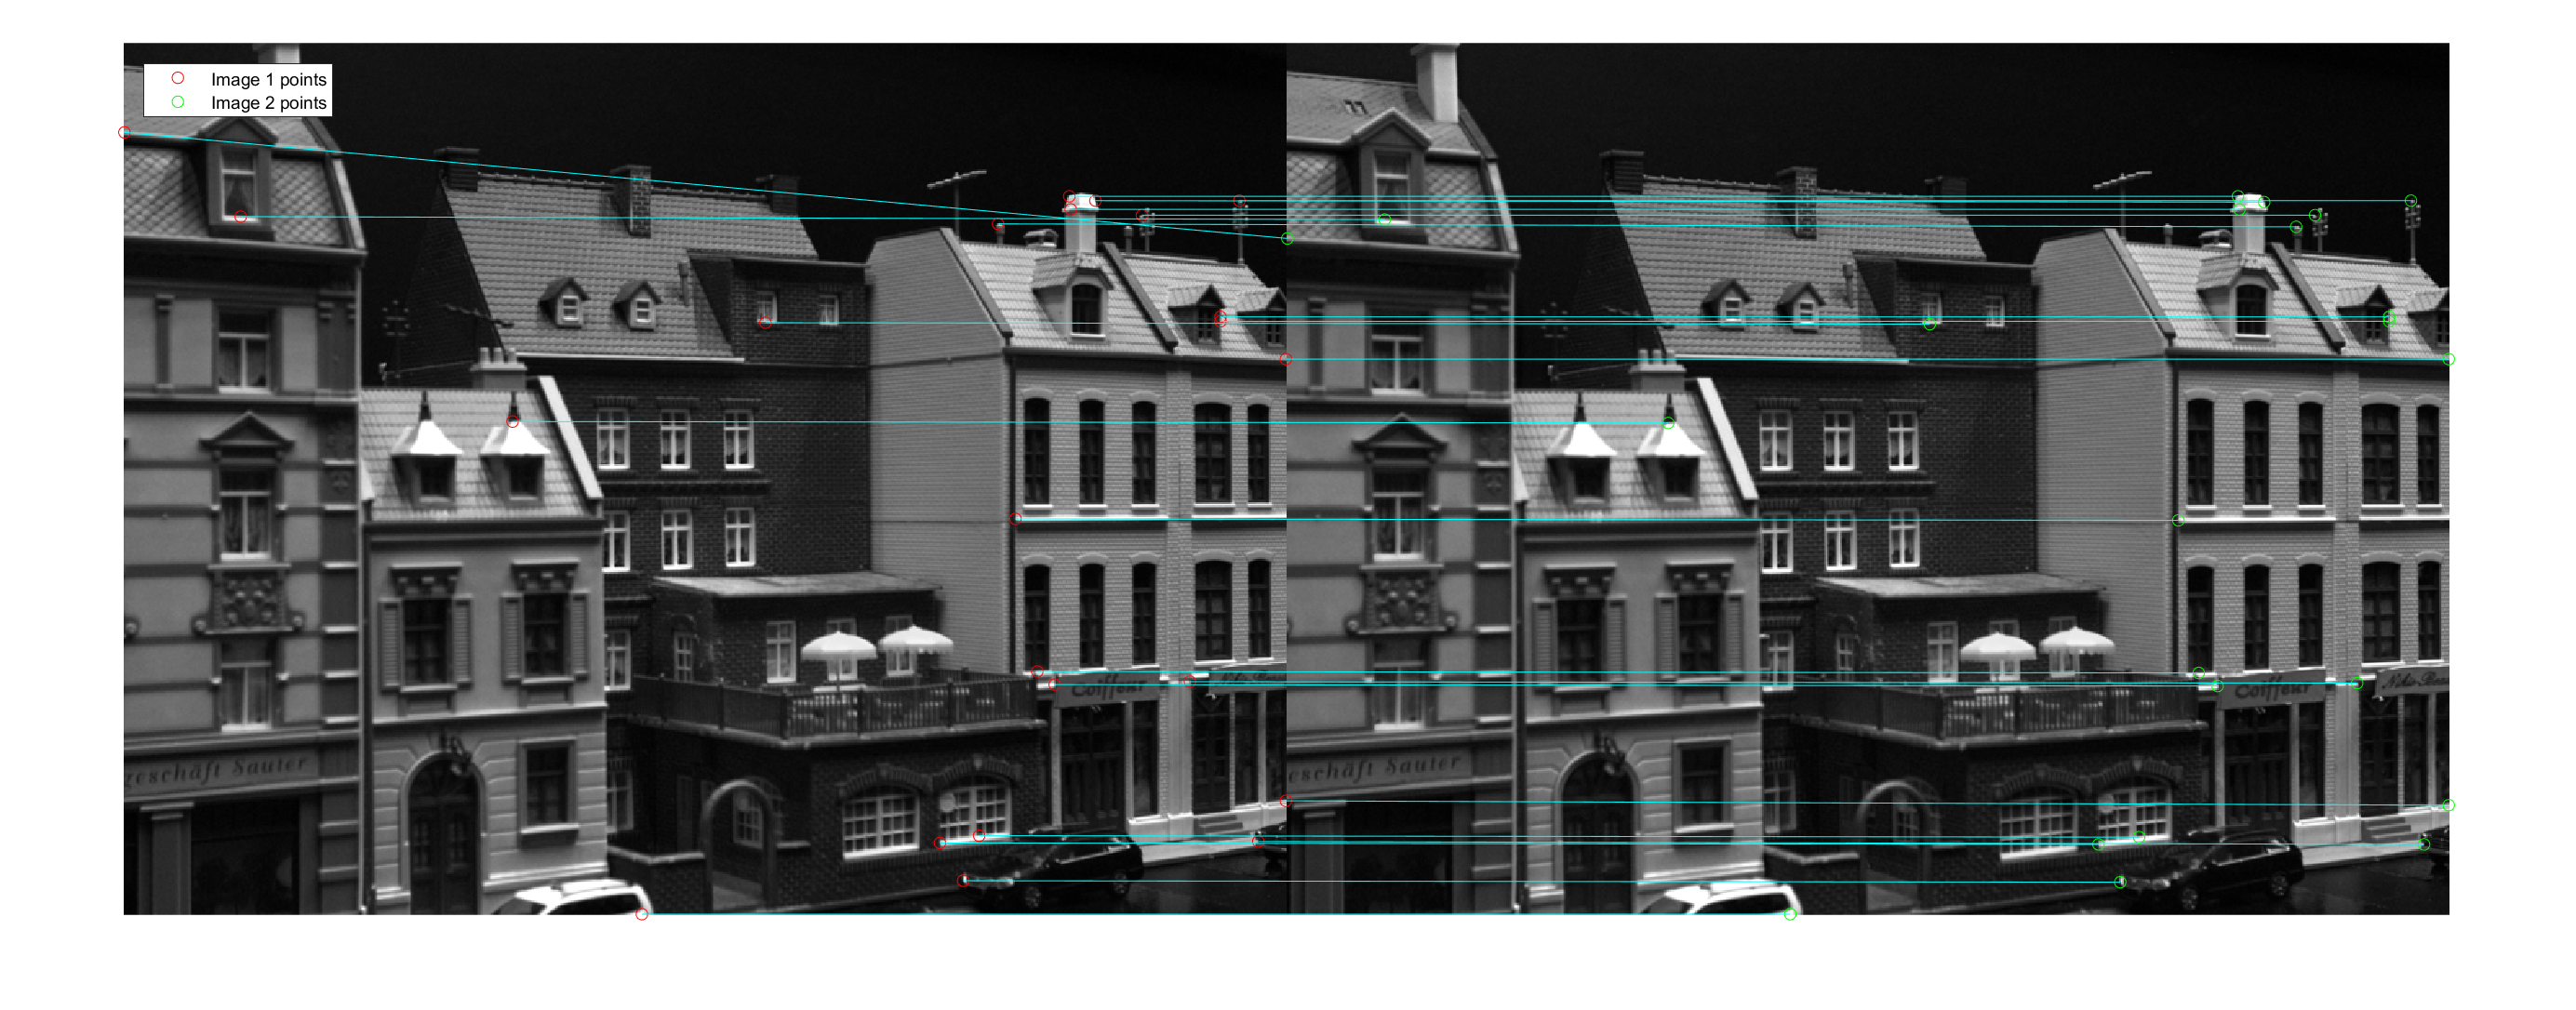
\includegraphics[width=\textwidth]{output/matches7.png}
	\caption{Using descriptor field width / height 7}
\end{subfigure}\\

Looking at the matches produced for descriptor sizes 5 and 7, it seems that very many matches have been filtered out. We will be able to see what filter-method caused most of this in the statistics section.\\
In both mathcing, we see one tilted line. This line is wrong; However, it may have something to do with the interest point being more or less on the edge of the image. Also the two matched points do look somewhat similar, both being placed in an edge of the roof and all.\\
The rest of the lines are fairly parallel, which is a good sign.

\end{figure}
\begin{figure}[H]
\ContinuedFloat
\begin{subfigure}[b]{1\textwidth}
	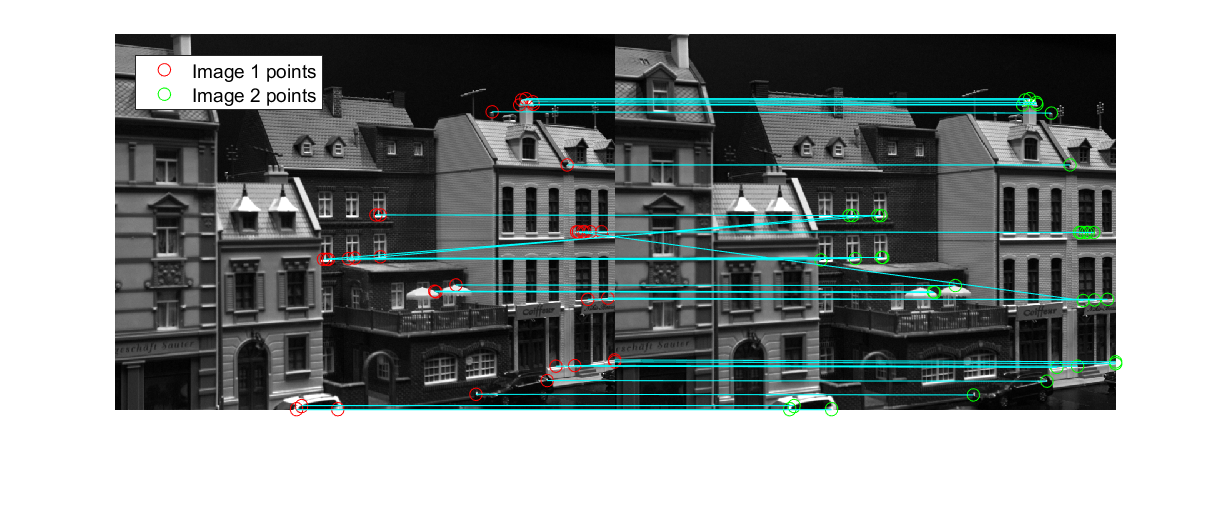
\includegraphics[width=\textwidth]{output/matches9.png}
	\caption{Using descriptor field width / height 9}
\end{subfigure}\\
\begin{subfigure}[b]{1\textwidth}
	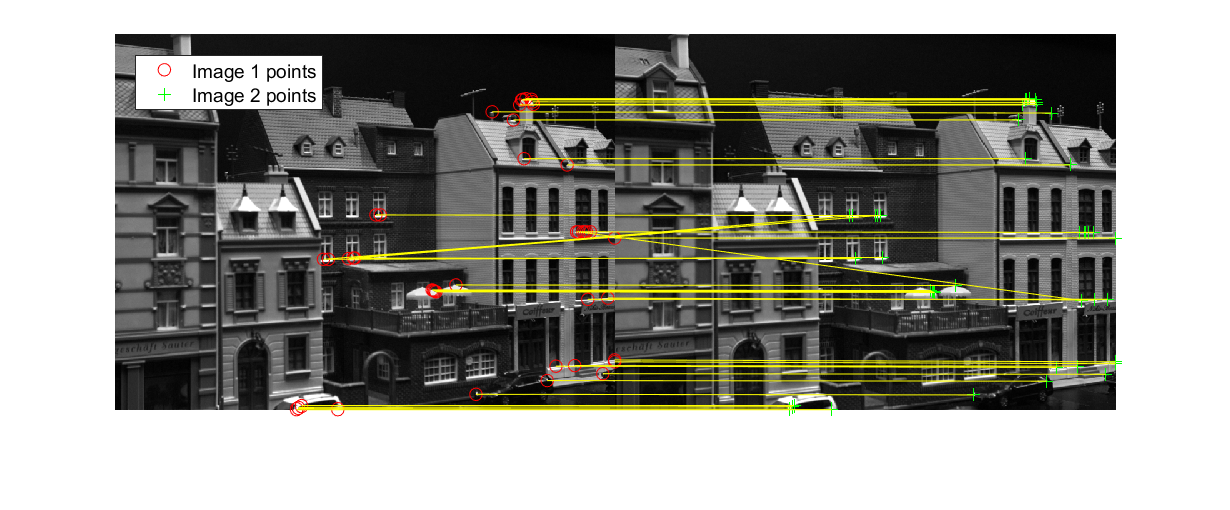
\includegraphics[width=\textwidth]{output/matches13.png}
	\caption{Using descriptor field width / height 13}
\end{subfigure}
\end{figure}

For the matches produced by descriptor size 9 there are only parallel lines. In the case of descriptor size 13, there is a single tilted line, which again is some edge case.\\
There seem to be a lot more matches being accepted for "9" and "13".\\
We will look at what the reason for this is in the statistics section.\\
Lastly, it seems that only the case of descriptor size 13 managed to \textit{not} match the wrong two "chimney-things" in the top-right.\\

\textbf{Statistics}\\
In table \ref{tab:stats} we see the statistics of our matching. We made 170382 comparisons in total, and we had 389 and 438 interest points in image 1 and 2 respectively. We can see that the first filtering we do reduced the number of possible correspondences significantly. We discard more points for small $N$ because we only have a little neighborhood. The "pattern"\ of the neighborhood is more likely to be seen in other parts of the image, whereas larger neighborhoods are more "complex"\ and thus "rarer".\\
The number of potential matches is reduces even further when we check that a match from point $y$ to point $x$ is two-sided. Again we see that for the larger $N$ we have more potential matches than for small $N$. This is natural since the more potential matches we have, the higher the chance of them being true matches.\\
As we theorized the final thresholding does not have a noteworthy effect. The hard threshold we used was 100000. The thresholding seems to have a larger effect on large $N$ and practically none on the smaller. This is because the sum of squared intensity differences of  the smaller window sizes cannot sum up to the threshold, unless the best matching descriptors are still very different, in which case they should have been discarded during the first filtering. Therefore the hard threshold should probably have been chosen based on $N$.
\begin{table}[H]
	\centering
	\begin{tabular}{c||c|c|c|c}
		N & 5 & 7 & 9 & 13\\ \hline \hline
		Number of interest points, image 1 & 389 & 389 & 389 & 389 \\ \hline
		Number of interest points, image 2 & 438 & 438 & 438 & 438 \\ \hline
		Number of correspondences after filtering, image 1 & 31 & 34 & 46 & 61 \\\hline
		Number of correspondences after filtering, image 2 & 35 & 51 & 59 & 65 \\\hline
		Number of two-way accepted correspondences& 18 & 23 & 35 & 51 \\ \hline
		Number of correspondences after thresholding & 18 & 23 & 35 & 50 \\ \hline
		Worst possible dissimilarity between patches & 1625625 & 3186225 & 5267025 & 10989225 \\ \hline
		Average dissimilarity & 1330 & 3891.4 & 9511.1 & 2376 \\ \hline
		Standard deviation & 1300.5 & 3753.6 & 8151.8 & 2055.5 \\ \hline
	\end{tabular}
	\caption{Statistics of matching}
	\label{tab:stats}
\end{table}
We would like to have a small average dissimilarity, since small dissimilarity means that two points are a good match. We would also like for the standard deviation to be small, since we would like for all of our matchings to be good. A large standard deviation could mean that we have a few exceptionally good matchings or a few exceptionally bad matchings. From the means and standard deviations we see in table \ref{tab:stats} we can see that we do not get consistently good/bad matches. However the matches we do get seems to be very good, if we take into consideration the worst possible dissimilarity between two patches, calculated by $255^2N^2$. Based on worst case scenario, average dissimilarity, standard deviation and number of accepted matches, it would seem that a very large patch sizes yield the best true case to worst case ratio. This is again because large patches are more difficult to find at other image positions.

\end{homeworkSubProblem}

\end{homeworkProblem}

\end{document}